\documentclass[]{article}
\usepackage{lmodern}
\usepackage{amssymb,amsmath}
\usepackage{ifxetex,ifluatex}
\usepackage{fixltx2e} % provides \textsubscript
\ifnum 0\ifxetex 1\fi\ifluatex 1\fi=0 % if pdftex
  \usepackage[T1]{fontenc}
  \usepackage[utf8]{inputenc}
\else % if luatex or xelatex
  \ifxetex
    \usepackage{mathspec}
  \else
    \usepackage{fontspec}
  \fi
  \defaultfontfeatures{Ligatures=TeX,Scale=MatchLowercase}
\fi
% use upquote if available, for straight quotes in verbatim environments
\IfFileExists{upquote.sty}{\usepackage{upquote}}{}
% use microtype if available
\IfFileExists{microtype.sty}{%
\usepackage{microtype}
\UseMicrotypeSet[protrusion]{basicmath} % disable protrusion for tt fonts
}{}
\usepackage[margin=1in]{geometry}
\usepackage{hyperref}
\hypersetup{unicode=true,
            pdftitle={Chapter 8 - Introduction to Linear Regression HomeWork\_8},
            pdfauthor={Salma Elshahawy},
            pdfborder={0 0 0},
            breaklinks=true}
\urlstyle{same}  % don't use monospace font for urls
\usepackage{color}
\usepackage{fancyvrb}
\newcommand{\VerbBar}{|}
\newcommand{\VERB}{\Verb[commandchars=\\\{\}]}
\DefineVerbatimEnvironment{Highlighting}{Verbatim}{commandchars=\\\{\}}
% Add ',fontsize=\small' for more characters per line
\usepackage{framed}
\definecolor{shadecolor}{RGB}{248,248,248}
\newenvironment{Shaded}{\begin{snugshade}}{\end{snugshade}}
\newcommand{\AlertTok}[1]{\textcolor[rgb]{0.94,0.16,0.16}{#1}}
\newcommand{\AnnotationTok}[1]{\textcolor[rgb]{0.56,0.35,0.01}{\textbf{\textit{#1}}}}
\newcommand{\AttributeTok}[1]{\textcolor[rgb]{0.77,0.63,0.00}{#1}}
\newcommand{\BaseNTok}[1]{\textcolor[rgb]{0.00,0.00,0.81}{#1}}
\newcommand{\BuiltInTok}[1]{#1}
\newcommand{\CharTok}[1]{\textcolor[rgb]{0.31,0.60,0.02}{#1}}
\newcommand{\CommentTok}[1]{\textcolor[rgb]{0.56,0.35,0.01}{\textit{#1}}}
\newcommand{\CommentVarTok}[1]{\textcolor[rgb]{0.56,0.35,0.01}{\textbf{\textit{#1}}}}
\newcommand{\ConstantTok}[1]{\textcolor[rgb]{0.00,0.00,0.00}{#1}}
\newcommand{\ControlFlowTok}[1]{\textcolor[rgb]{0.13,0.29,0.53}{\textbf{#1}}}
\newcommand{\DataTypeTok}[1]{\textcolor[rgb]{0.13,0.29,0.53}{#1}}
\newcommand{\DecValTok}[1]{\textcolor[rgb]{0.00,0.00,0.81}{#1}}
\newcommand{\DocumentationTok}[1]{\textcolor[rgb]{0.56,0.35,0.01}{\textbf{\textit{#1}}}}
\newcommand{\ErrorTok}[1]{\textcolor[rgb]{0.64,0.00,0.00}{\textbf{#1}}}
\newcommand{\ExtensionTok}[1]{#1}
\newcommand{\FloatTok}[1]{\textcolor[rgb]{0.00,0.00,0.81}{#1}}
\newcommand{\FunctionTok}[1]{\textcolor[rgb]{0.00,0.00,0.00}{#1}}
\newcommand{\ImportTok}[1]{#1}
\newcommand{\InformationTok}[1]{\textcolor[rgb]{0.56,0.35,0.01}{\textbf{\textit{#1}}}}
\newcommand{\KeywordTok}[1]{\textcolor[rgb]{0.13,0.29,0.53}{\textbf{#1}}}
\newcommand{\NormalTok}[1]{#1}
\newcommand{\OperatorTok}[1]{\textcolor[rgb]{0.81,0.36,0.00}{\textbf{#1}}}
\newcommand{\OtherTok}[1]{\textcolor[rgb]{0.56,0.35,0.01}{#1}}
\newcommand{\PreprocessorTok}[1]{\textcolor[rgb]{0.56,0.35,0.01}{\textit{#1}}}
\newcommand{\RegionMarkerTok}[1]{#1}
\newcommand{\SpecialCharTok}[1]{\textcolor[rgb]{0.00,0.00,0.00}{#1}}
\newcommand{\SpecialStringTok}[1]{\textcolor[rgb]{0.31,0.60,0.02}{#1}}
\newcommand{\StringTok}[1]{\textcolor[rgb]{0.31,0.60,0.02}{#1}}
\newcommand{\VariableTok}[1]{\textcolor[rgb]{0.00,0.00,0.00}{#1}}
\newcommand{\VerbatimStringTok}[1]{\textcolor[rgb]{0.31,0.60,0.02}{#1}}
\newcommand{\WarningTok}[1]{\textcolor[rgb]{0.56,0.35,0.01}{\textbf{\textit{#1}}}}
\usepackage{graphicx,grffile}
\makeatletter
\def\maxwidth{\ifdim\Gin@nat@width>\linewidth\linewidth\else\Gin@nat@width\fi}
\def\maxheight{\ifdim\Gin@nat@height>\textheight\textheight\else\Gin@nat@height\fi}
\makeatother
% Scale images if necessary, so that they will not overflow the page
% margins by default, and it is still possible to overwrite the defaults
% using explicit options in \includegraphics[width, height, ...]{}
\setkeys{Gin}{width=\maxwidth,height=\maxheight,keepaspectratio}
\IfFileExists{parskip.sty}{%
\usepackage{parskip}
}{% else
\setlength{\parindent}{0pt}
\setlength{\parskip}{6pt plus 2pt minus 1pt}
}
\setlength{\emergencystretch}{3em}  % prevent overfull lines
\providecommand{\tightlist}{%
  \setlength{\itemsep}{0pt}\setlength{\parskip}{0pt}}
\setcounter{secnumdepth}{0}
% Redefines (sub)paragraphs to behave more like sections
\ifx\paragraph\undefined\else
\let\oldparagraph\paragraph
\renewcommand{\paragraph}[1]{\oldparagraph{#1}\mbox{}}
\fi
\ifx\subparagraph\undefined\else
\let\oldsubparagraph\subparagraph
\renewcommand{\subparagraph}[1]{\oldsubparagraph{#1}\mbox{}}
\fi

%%% Use protect on footnotes to avoid problems with footnotes in titles
\let\rmarkdownfootnote\footnote%
\def\footnote{\protect\rmarkdownfootnote}

%%% Change title format to be more compact
\usepackage{titling}

% Create subtitle command for use in maketitle
\providecommand{\subtitle}[1]{
  \posttitle{
    \begin{center}\large#1\end{center}
    }
}

\setlength{\droptitle}{-2em}

  \title{Chapter 8 - Introduction to Linear Regression HomeWork\_8}
    \pretitle{\vspace{\droptitle}\centering\huge}
  \posttitle{\par}
    \author{Salma Elshahawy}
    \preauthor{\centering\large\emph}
  \postauthor{\par}
    \date{}
    \predate{}\postdate{}
  
\usepackage{geometry}
\usepackage{multicol}
\usepackage{multirow}
\usepackage{xcolor}

\begin{document}
\maketitle

\textbf{Nutrition at Starbucks, Part I.} (8.22, p.~326) The scatterplot
below shows the relationship between the number of calories and amount
of carbohydrates (in grams) Starbucks food menu items contain. Since
Starbucks only lists the number of calories on the display items, we are
interested in predicting the amount of carbs a menu item has based on
its calorie content.

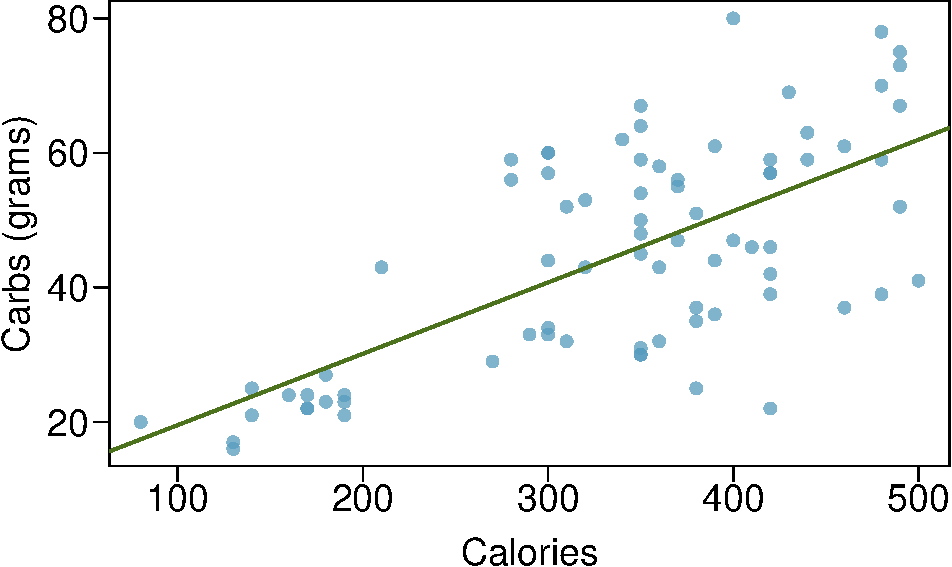
\includegraphics[width=0.33\linewidth]{Homework_8_files/figure-latex/unnamed-chunk-1-1}
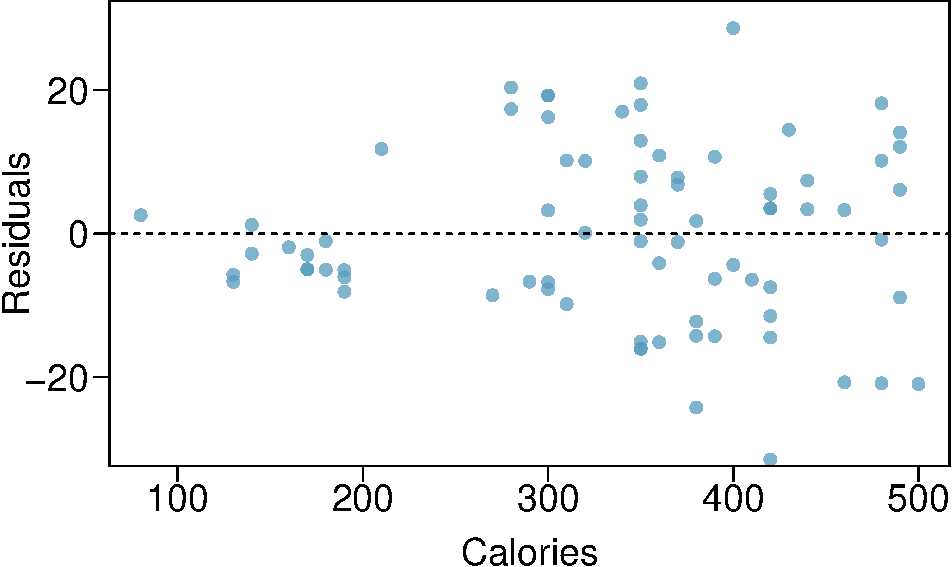
\includegraphics[width=0.33\linewidth]{Homework_8_files/figure-latex/unnamed-chunk-1-2}
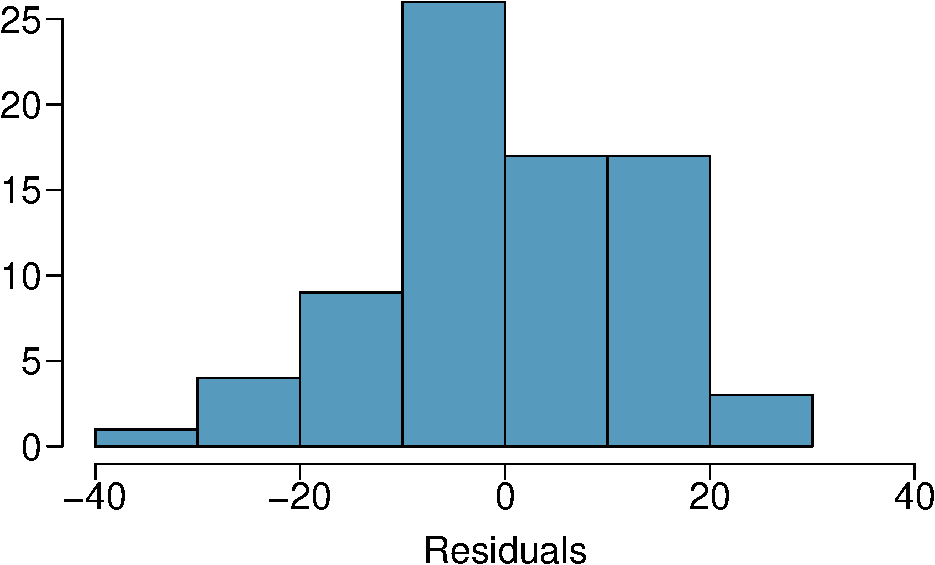
\includegraphics[width=0.33\linewidth]{Homework_8_files/figure-latex/unnamed-chunk-1-3}

\begin{enumerate}
\def\labelenumi{(\alph{enumi})}
\tightlist
\item
  Describe the relationship between number of calories and amount of
  carbohydrates (in grams) that Starbucks food menu items contain.
\end{enumerate}

\emph{The relationship between calories and amount of carbo seems to be
linear but not strong}

\begin{enumerate}
\def\labelenumi{(\alph{enumi})}
\setcounter{enumi}{1}
\tightlist
\item
  In this scenario, what are the explanatory and response variables?
\end{enumerate}

\emph{The explanatory is Calories, and the response variable is Carbs}

\begin{enumerate}
\def\labelenumi{(\alph{enumi})}
\setcounter{enumi}{2}
\tightlist
\item
  Why might we want to fit a regression line to these data?
\end{enumerate}

\emph{We need to do that to have a prediction of the amount of Carbs in
the response variable}

\begin{enumerate}
\def\labelenumi{(\alph{enumi})}
\setcounter{enumi}{3}
\tightlist
\item
  Do these data meet the conditions required for fitting a least squares
  line?
\end{enumerate}

\emph{Linearity = \textgreater{} yes, it follows a normal distribution
according to histogram} \emph{Nearly normal residuals =\textgreater{}
faily yes;however the histogram is not symmetrical, this may opt out
this condition} \emph{Constant Variability =\textgreater{} The
variablility is not constant, where there are more residuals on the
rightside of the scatter plot} \emph{I don't think that this model can
fit the regression model due to lack of variance and unsymmetrical
residuals}

\begin{center}\rule{0.5\linewidth}{\linethickness}\end{center}

\clearpage

\textbf{Body measurements, Part I.} (8.13, p.~316) Researchers studying
anthropometry collected body girth measurements and skeletal diameter
measurements, as well as age, weight, height and gender for 507
physically active individuals.19 The scatterplot below shows the
relationship between height and shoulder girth (over deltoid muscles),
both measured in centimeters.

\begin{center}

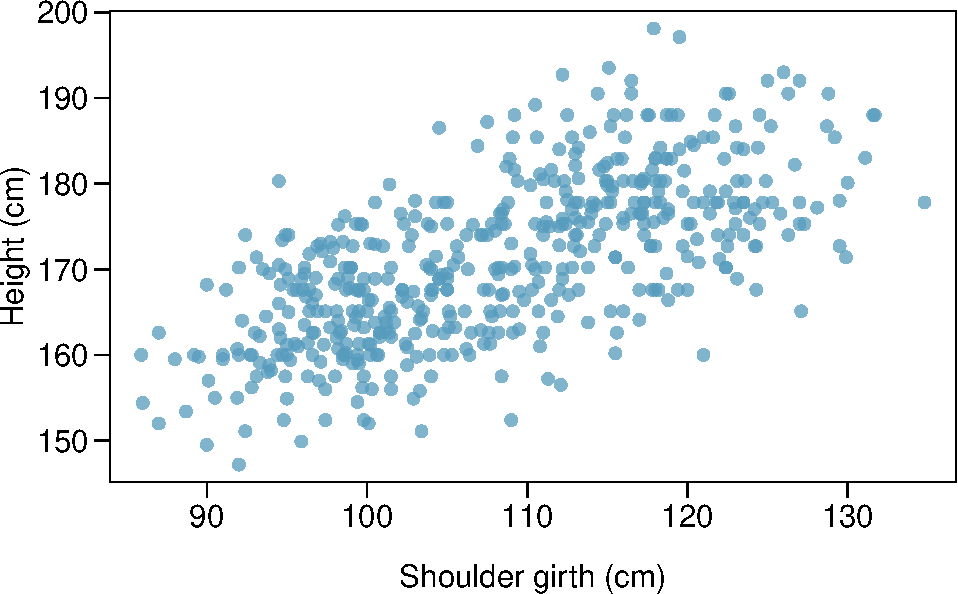
\includegraphics[width=0.5\linewidth]{Homework_8_files/figure-latex/unnamed-chunk-2-1} 
\end{center}

\begin{enumerate}
\def\labelenumi{(\alph{enumi})}
\tightlist
\item
  Describe the relationship between shoulder girth and height.
\end{enumerate}

\emph{The relationship seems to be linear}

\begin{enumerate}
\def\labelenumi{(\alph{enumi})}
\setcounter{enumi}{1}
\tightlist
\item
  How would the relationship change if shoulder girth was measured in
  inches while the units of height remained in centimeters?
\end{enumerate}

\emph{It should remain the same; however the points will be more
squished to the left}

\begin{center}\rule{0.5\linewidth}{\linethickness}\end{center}

\clearpage

\textbf{Body measurements, Part III.} (8.24, p.~326) Exercise above
introduces data on shoulder girth and height of a group of individuals.
The mean shoulder girth is 107.20 cm with a standard deviation of 10.37
cm. The mean height is 171.14 cm with a standard deviation of 9.41 cm.
The correlation between height and shoulder girth is 0.67.

\begin{enumerate}
\def\labelenumi{(\alph{enumi})}
\tightlist
\item
  Write the equation of the regression line for predicting height.
\end{enumerate}

\(\widehat{ x } =\quad 107.2\\ \bar{ y } =\quad 171.14\\ { s }_{ \bar{ x } }=\quad 10.37\\ { s }_{ \bar{ y } }=\quad 9.41\\ { R } =\quad 0.67\)
\(b1\quad =\quad \frac { { s }_{ \bar{ y } } }{ { s }_{ \bar{ x } } } *{ R }\)
\(b1\quad =\quad \frac { 9.41 }{ 10.37 } *\quad 0.67\)
\((y-\bar{ y } )\quad =\quad b1(x-\bar{ x } )\)
\((y-171.14)\quad =\quad 6.9479*(x-107.2)\)

\emph{The equation of regression will be:}

\(y\quad =\quad 105.965\quad +\quad 0.607*x\)
\(height\quad =\quad 105.965\quad +\quad 0.607*shoulder\quad girth\)

\begin{enumerate}
\def\labelenumi{(\alph{enumi})}
\setcounter{enumi}{1}
\tightlist
\item
  Interpret the slope and the intercept in this context.
\end{enumerate}

\emph{The slope is: 0.607 means that to increase height, the shoulder
length should be increased by this slope which is 0.607} \emph{The
intercept: for a shoulder girth of 0 cm, the average height increases by
105.965 cm}

\begin{enumerate}
\def\labelenumi{(\alph{enumi})}
\setcounter{enumi}{2}
\tightlist
\item
  Calculate \(R^2\) of the regression line for predicting height from
  shoulder girth, and interpret it in the context of the application.
\end{enumerate}

\({ { R } }^{ 2 }\quad =\quad { 0.67 }^{ 2 }\\ { { R } }^{ 2 }\quad =\quad 0.4489\)

\emph{44.89\% of the variation in height is explained by shoulder girth}

\begin{enumerate}
\def\labelenumi{(\alph{enumi})}
\setcounter{enumi}{3}
\tightlist
\item
  A randomly selected student from your class has a shoulder girth of
  100 cm. Predict the height of this student using the model.
\end{enumerate}

\(height\quad =\quad 105.965\quad +\quad 0.607*100\)
\(height\quad =\quad 166.762\)

\emph{The height should be 166.76}

\begin{enumerate}
\def\labelenumi{(\alph{enumi})}
\setcounter{enumi}{4}
\tightlist
\item
  The student from part (d) is 160 cm tall. Calculate the residual, and
  explain what this residual means.
\end{enumerate}

\({ e }_{ i }\quad =\quad { y }_{ i }-\bar{ y } \\ { e }_{ i }\quad =\quad 160\quad -\quad 166.76\\ { e }_{ i }\quad =\quad -6.76\)

\emph{This means by a negative sign that the model overestimated the
height by 6.76}

\begin{enumerate}
\def\labelenumi{(\alph{enumi})}
\setcounter{enumi}{5}
\tightlist
\item
  A one year old has a shoulder girth of 56 cm. Would it be appropriate
  to use this linear model to predict the height of this child?
\end{enumerate}

\emph{the average shoulder girth for this sample is 107.2 which means
that 56 point will be far away. So I think that we cannot use this model
to predict such prediction}

\begin{center}\rule{0.5\linewidth}{\linethickness}\end{center}

\clearpage

\textbf{Cats, Part I.} (8.26, p.~327) The following regression output is
for predicting the heart weight (in g) of cats from their body weight
(in kg). The coefficients are estimated using a dataset of 144 domestic
cats.

\begin{center}
{
\begin{tabular}{rrrrr}
    \hline
            & Estimate  & Std. Error    & t value   & Pr($>$$|$t$|$) \\ 
    \hline
(Intercept) & -0.357    & 0.692         & -0.515    & 0.607 \\ 
body wt     & 4.034     & 0.250         & 16.119    & 0.000 \\ 
    \hline
\end{tabular} \ \\
$s = 1.452 \qquad R^2 = 64.66\% \qquad R^2_{adj} = 64.41\%$ 
}
\end{center}

\begin{center}

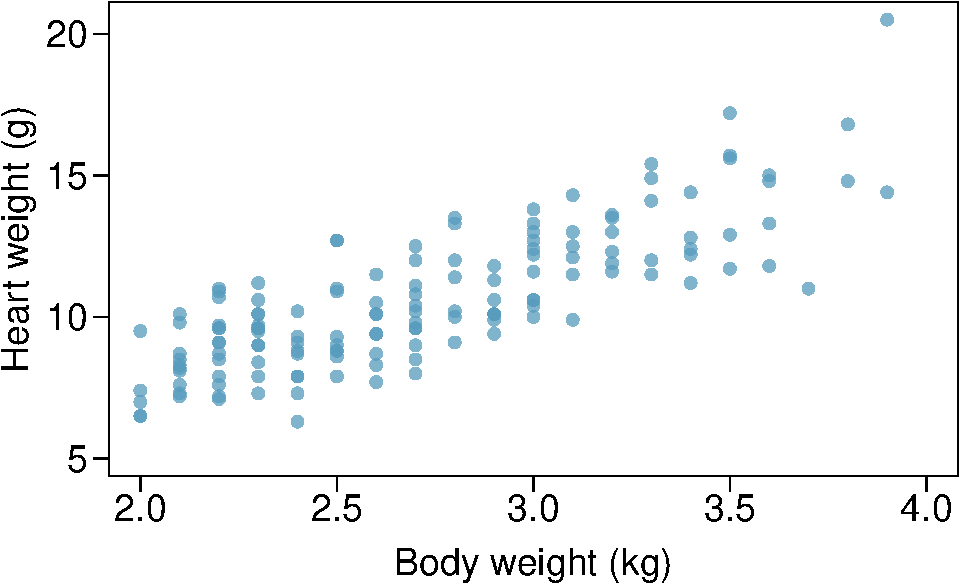
\includegraphics[width=0.5\linewidth]{Homework_8_files/figure-latex/unnamed-chunk-3-1} 
\end{center}

\begin{enumerate}
\def\labelenumi{(\alph{enumi})}
\tightlist
\item
  Write out the linear model.
\end{enumerate}

\emph{heart\_weight = -0.357 + 4.034 * body\_weight }

\begin{enumerate}
\def\labelenumi{(\alph{enumi})}
\setcounter{enumi}{1}
\tightlist
\item
  Interpret the intercept.
\end{enumerate}

\emph{Intercept means that for body weight 0, the average heart weight
is -0.357 grams}

\begin{enumerate}
\def\labelenumi{(\alph{enumi})}
\setcounter{enumi}{2}
\tightlist
\item
  Interpret the slope.
\end{enumerate}

\emph{The slope means that to increase heart\_weight , the body weight
should be increased by 4.035}

\begin{enumerate}
\def\labelenumi{(\alph{enumi})}
\setcounter{enumi}{3}
\tightlist
\item
  Interpret \(R^2\).
\end{enumerate}

\emph{64\% R-squared means that the variablility in heart weight of cats
can be explained by body\_weight}

\begin{enumerate}
\def\labelenumi{(\alph{enumi})}
\setcounter{enumi}{4}
\tightlist
\item
  Calculate the correlation coefficient.
\end{enumerate}

\begin{Shaded}
\begin{Highlighting}[]
\NormalTok{R <-}\StringTok{ }\KeywordTok{sqrt}\NormalTok{(}\FloatTok{0.6466}\NormalTok{)}
\NormalTok{R}
\end{Highlighting}
\end{Shaded}

\begin{verbatim}
## [1] 0.8041144
\end{verbatim}

\begin{center}\rule{0.5\linewidth}{\linethickness}\end{center}

\clearpage

\textbf{Rate my professor.} (8.44, p.~340) Many college courses conclude
by giving students the opportunity to evaluate the course and the
instructor anonymously. However, the use of these student evaluations as
an indicator of course quality and teaching effectiveness is often
criticized because these measures may reflect the influence of
non-teaching related characteristics, such as the physical appearance of
the instructor. Researchers at University of Texas, Austin collected
data on teaching evaluation score (higher score means better) and
standardized beauty score (a score of 0 means average, negative score
means below average, and a positive score means above average) for a
sample of 463 professors. The scatterplot below shows the relationship
between these variables, and also provided is a regression output for
predicting teaching evaluation score from beauty score.

\begin{center}
\begin{tabular}{rrrrr}
    \hline
            & Estimate  & Std. Error    & t value   & Pr($>$$|$t$|$) \\ 
  \hline
(Intercept) & 4.010     & 0.0255        &   157.21  & 0.0000 \\ 
beauty      &  \fbox{\textcolor{white}{{ Cell 1}}}  
                        & 0.0322        & 4.13      & 0.0000\vspace{0.8mm} \\ 
   \hline
\end{tabular}



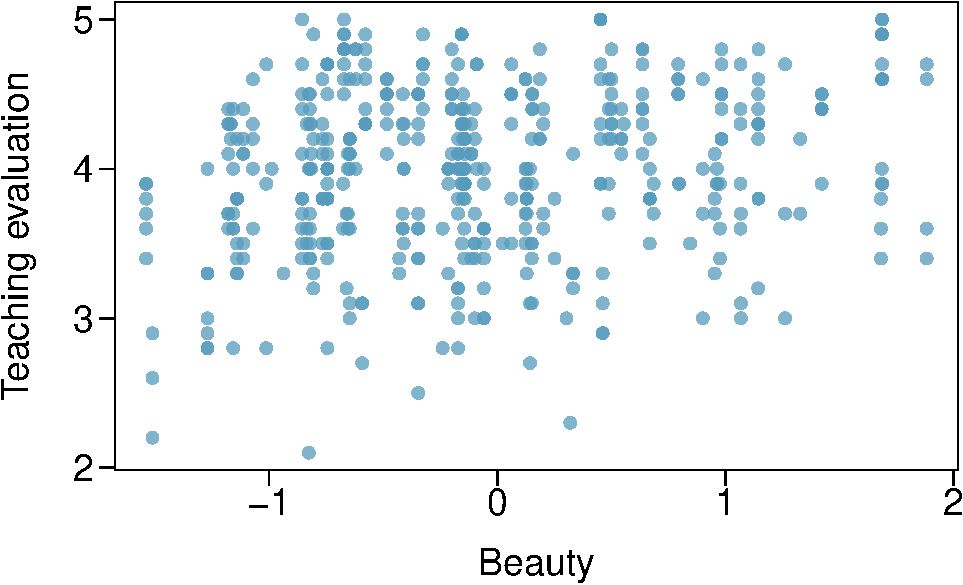
\includegraphics[width=0.5\linewidth]{Homework_8_files/figure-latex/unnamed-chunk-5-1} 
\end{center}

\begin{enumerate}
\def\labelenumi{(\alph{enumi})}
\tightlist
\item
  Given that the average standardized beauty score is -0.0883 and
  average teaching evaluation score is 3.9983, calculate the slope.
  Alternatively, the slope may be computed using just the information
  provided in the model summary table.
\end{enumerate}

\emph{considered that both x-hat and y-hat both located on the
regression line, we can have the following equation of the regression
line}

\begin{Shaded}
\begin{Highlighting}[]
\NormalTok{slope <-}\StringTok{ }\NormalTok{(}\FloatTok{3.9983} \OperatorTok{-}\StringTok{ }\FloatTok{4.010}\NormalTok{)}\OperatorTok{/}\NormalTok{(}\OperatorTok{-}\FloatTok{0.0883}\NormalTok{)}
\NormalTok{slope}
\end{Highlighting}
\end{Shaded}

\begin{verbatim}
## [1] 0.1325028
\end{verbatim}

\begin{enumerate}
\def\labelenumi{(\alph{enumi})}
\setcounter{enumi}{1}
\tightlist
\item
  Do these data provide convincing evidence that the slope of the
  relationship between teaching evaluation and beauty is positive?
  Explain your reasoning.
\end{enumerate}

\emph{Since the slope is positive the relationship is positive. If we
set up a hypothesis test with
\({ H }_{ 0 }\quad :\quad { \beta }_{ 1 }\quad =\quad 0\quad and\quad \\ { H }_{ A }\quad :\quad { \beta }_{ 1 }\quad >\quad 0\),
then based on the summary table the p−value is nearly 0. And this is for
a two-sided test, so it'll be even closer to 0 for a one-sided test. We
reject the null hypothesis. There is convincing evidence that the
relationship between teaching evluation and beauty is positive.}

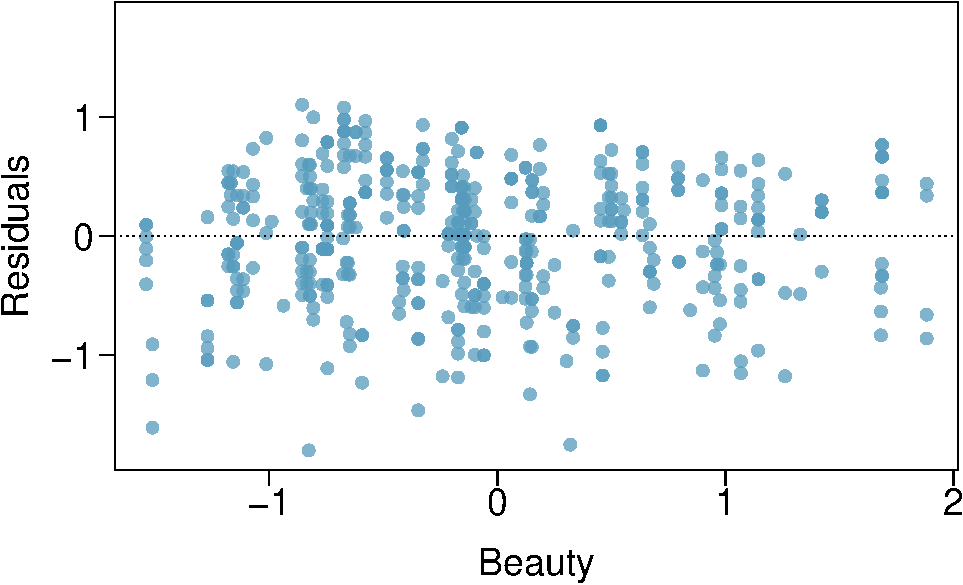
\includegraphics[width=0.5\linewidth]{Homework_8_files/figure-latex/unnamed-chunk-7-1}
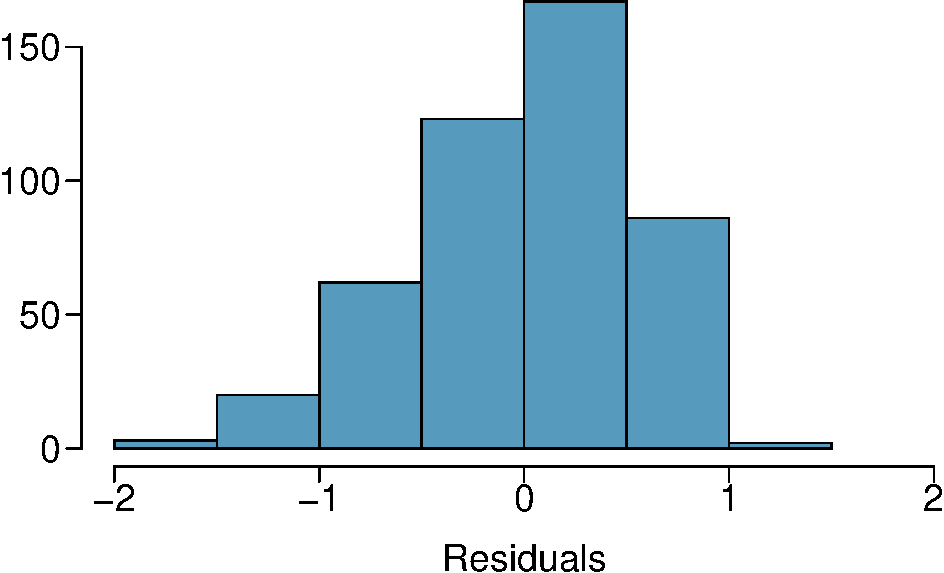
\includegraphics[width=0.5\linewidth]{Homework_8_files/figure-latex/unnamed-chunk-7-2}
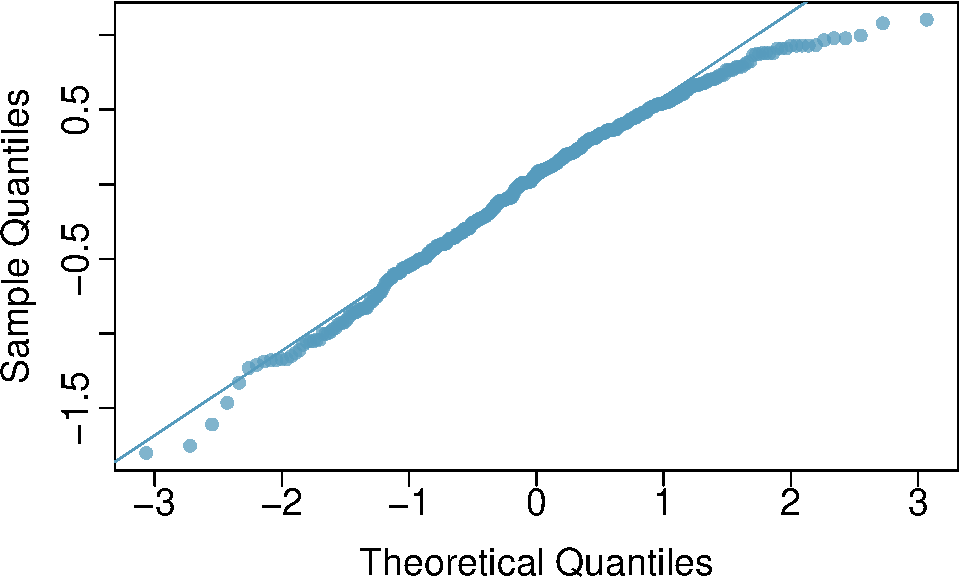
\includegraphics[width=0.5\linewidth]{Homework_8_files/figure-latex/unnamed-chunk-7-3}
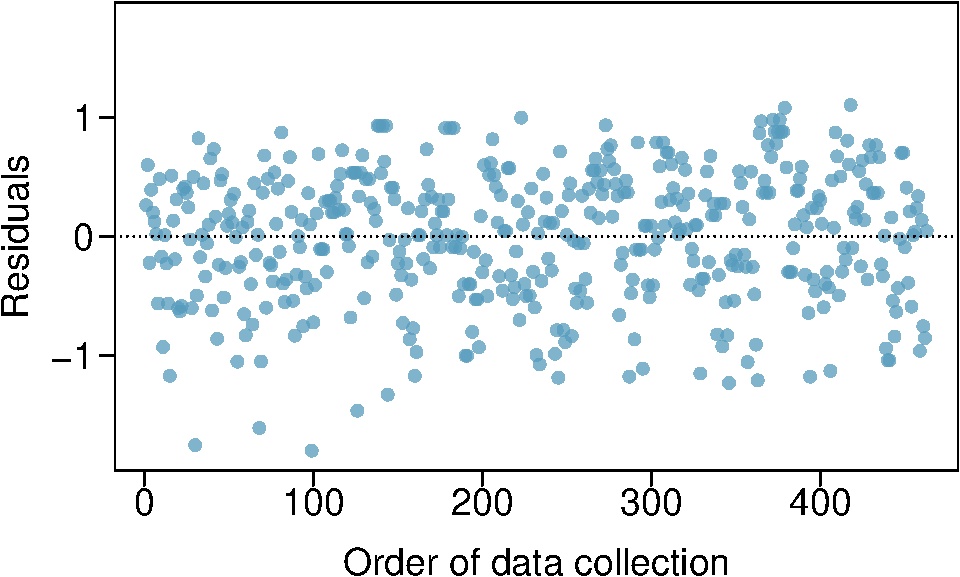
\includegraphics[width=0.5\linewidth]{Homework_8_files/figure-latex/unnamed-chunk-7-4}

\begin{enumerate}
\def\labelenumi{(\alph{enumi})}
\setcounter{enumi}{2}
\tightlist
\item
  List the conditions required for linear regression and check if each
  one is satisfied for this model based on the following diagnostic
  plots.
\end{enumerate}

\emph{Linearity: Based on the scatterplot, there may be a weak linear
relationship. There is no evident pattern in the residual plot. Nearly
normal residuals: The histogram of the residuals exhibits a left skew.
Additionally, the points seem to move away from the normal probability
line on each end. However, the bulk of the data is very close to the
line. I would conclude that the distribution of residuals is nearly
normal. Constant variability: Based on residual plot, there appears to
be constant variability in the data. Independent observations:
Observations are not a time series, and can be assumed to be independent
(unless there is evidence that students copied each other's
evaluations). I believe all conditions are satisfied for this linear
model.}


\end{document}
